\documentclass[a4paper,12pt]{report}
\usepackage{graphicx}
\title{Report\\``MTSK-GAME''}

\author{Pietro Olivi\\
Leonardo Tassinari\\
Lorenzo Dalmonte\\
Alessio Paoloni}
\date{\today}


\begin{document}

\maketitle

\tableofcontents

\chapter{Analysis}
The software commissioned by the teachers of the Object Oriented Pro\-gramming course aims to create an application designed to enhance psycho-motor skills through a gaming experience based on multitasking.\\
The term \textit{Multitasking} refers to the ability of a person or a product to do more than one thing at a time.

\section{Requirements}
\subsection*{Functional}
\begin{itemize}
	\item Upon starting, the software will display a simple minigame.\\
	A minigame is a never-ending challenge that requires simple actions from the player in order to keep the game going on.
	After a short amount of time a new minigame will show up and so on until all four minigames are displayed.
	The player's goal is to last as long as possible. After failing a minigame the application will display the final score.
	\item The software has to keep track of how long the player lasts in the current match in order to calculate the score.
\end{itemize}

\subsection*{Non functional}
\begin{itemize}
	\item The application shall sustain high framerate (around 120 fps) in all sections of the gameplay, even on older hardware\footnote{e.g. Intel Core i3 (fourth generation), 4Gb of RAM.}.
	\item It shall be possible to easily develop and swap the minigames among the ones that best fit the training purposes of the user on top of those already provided. 
\end{itemize}

\section{Domain analysis}

MTSK-Game shall display some \textit{minigames},
The provided minigames are:
\begin{itemize} 
	\item \textit{WhacAMole} where the player has to stomp appearing \textit{moles} before they get away.
	\item \textit{CatchTheSquare} where the player must collect \textit{squares} running over them with a \textit{circle} before they disappear.
	\item \textit{DodgeATriangle} where the player has to slide a \textit{rectangle} up and down, switching lanes to avoid hitting moving \textit{triangles}.
	\item \textit{FlappyBirdAlike} where the player needs to control a \textit{cursor} leading it to fit between \textit{obstacles} that will come towards it.
\end{itemize}
Upon user defeat, the \textit{score} will be shown.

\begin{figure}[h]
	\centering{}
	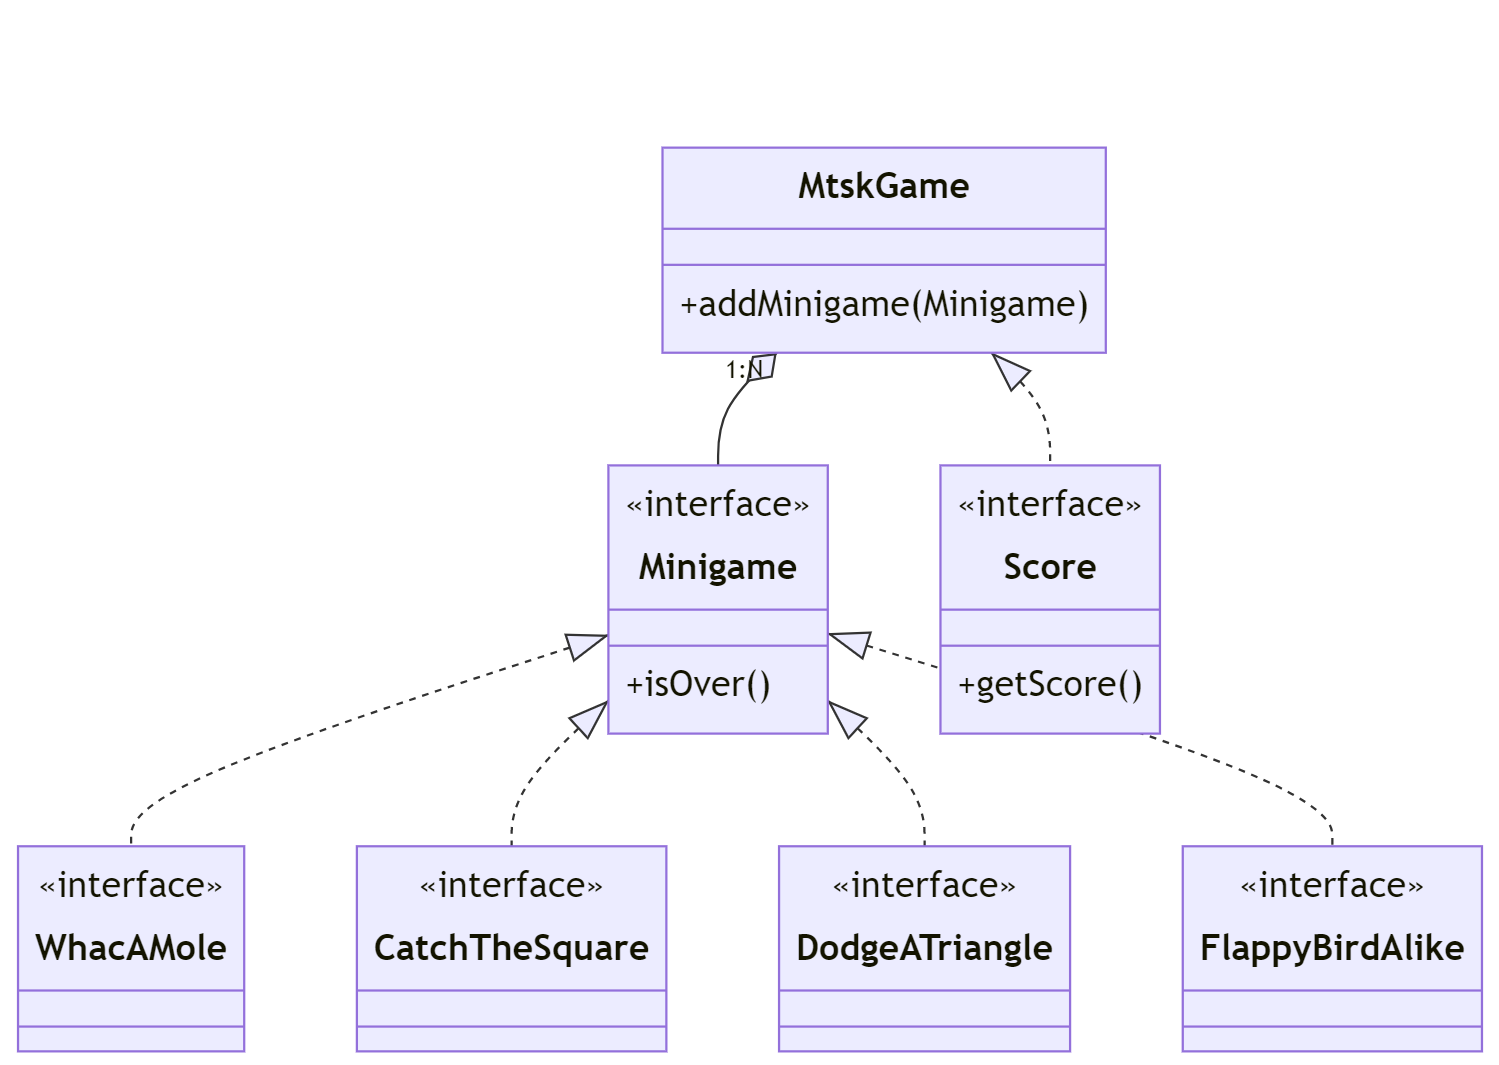
\includegraphics[width=\textwidth]{res/mermaid-diagram-2022-12-24-032504.png}
	\caption{UML diagram of the domain analysis}
\end{figure}

\chapter{Design}

\end{document}
